
\section{Implementation Details}

\subsection{Patch Match}

The main bottleneck of patch-based methods has long been the process of finding corresponding patches in the exemplar. Therefore comes Patch Match \cite{Barnes09}, a fast approximate nearest neighbor algorithm for image patches.
It is based on the \emph{coherence assumption}, namely that, while patches mapped from A to B can be mapped everywhere in B, nearby patches in A are usually mapped together in B.

\begin{figure}[h]
\centering
	\begin{subfigure}[t]{0.155\textwidth}
		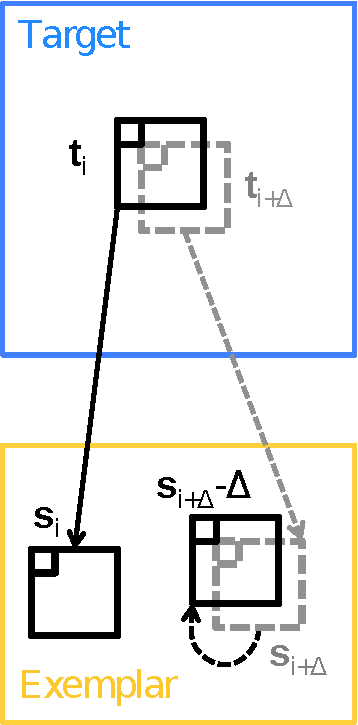
\includegraphics[width=\textwidth]{figures/propagation_text2}
		\caption{Propagation}
	\end{subfigure}
	\begin{subfigure}[t]{0.155\textwidth}
		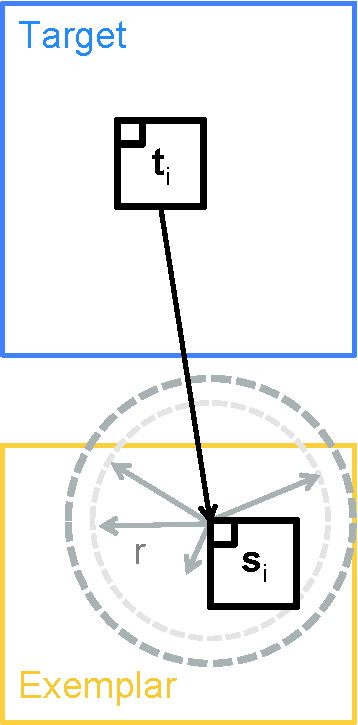
\includegraphics[width=\textwidth]{figures/randsearch_text}
		\caption{Random search}
	\end{subfigure}
	\begin{subfigure}[t]{0.155\textwidth}
		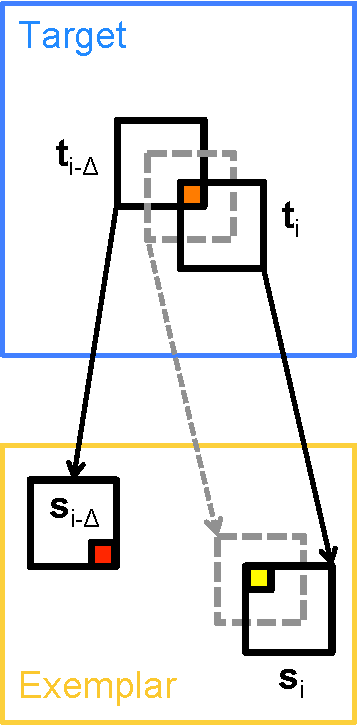
\includegraphics[width=\textwidth]{figures/voting_text}
		\caption{Voting}
	\end{subfigure}
   \caption{The main components of texture synthesis using Patch Match.}
\label{fig:texsynth_patchmatch}
\end{figure}

The algorithm proceeds in scanline-order from an initial guess of the nearest neighbor assignments $\{\ti \to \si\}$ and tries new candidate nearest neighbor patches using two main operations: \textbf{propagation} which tries to propagate the result of neighboring mappings, and \textbf{random search} that randomly samples patches in an exponentially decreasing window (see illustrations in Figure~\ref{fig:texsynth_patchmatch}).

\subsection{Extensions}

The Patch Match algorithm has been extended in several ways \cite{Barnes10} including the sampling of rotations, scales and mirrored patch spaces, the use of gain and bias adjustment (which Image Melding uses), a $k$-NN version of the algorithm as well as extra operations (enrichment and binning).

The voting step of texture optimization has also been explored with alternatives such as Meanshift \cite{Wexler07}, Histogram weighting \cite{Kopf07} as well as Bidirectional Similarity \cite{Simakov08}.

Finally, application-specific improvements have been made such as learning patch masks \cite{Kalantari14} or estimating the underlying geometry to search more efficiently \cite{Huang14}.

\subsection{Patch Web}

\subsection{Disparity}

\begin{enumerate}
	\item Compute constrained k-NNF from left to right
	\item Vote disparity
\end{enumerate}

Multiple voting strategies are possible:
\begin{itemize}
	\item Merge k-NNF into 1-NNF and then take naive patch shift as disparity
	\item Compute average disparity of $k \times N \times N$ overlapping patches
	\item Compute it with Mean-Shift
\end{itemize}

\TODO{Use patches with 5 channels: L, a, b, x, y}
\TODO{location of patch matters for disparity}

\TODO{talk about the missing "binning"}

\TODO{mention halfway domain}